%% LyX 2.3.6 created this file.  For more info, see http://www.lyx.org/.
%% Do not edit unless you really know what you are doing.
\documentclass[english,aspectratio=169]{beamer}
\usepackage{lmodern}
\renewcommand{\sfdefault}{lmss}
\renewcommand{\ttdefault}{lmtt}
\usepackage[T1]{fontenc}
\usepackage[latin9]{inputenc}
\setlength{\parskip}{\medskipamount}
\setlength{\parindent}{0pt}
\usepackage{amsbsy}
\usepackage{amssymb}
\usepackage{graphicx}
\PassOptionsToPackage{normalem}{ulem}
\usepackage{ulem}

\makeatletter

%%%%%%%%%%%%%%%%%%%%%%%%%%%%%% LyX specific LaTeX commands.
\pdfpageheight\paperheight
\pdfpagewidth\paperwidth


%%%%%%%%%%%%%%%%%%%%%%%%%%%%%% Textclass specific LaTeX commands.
% this default might be overridden by plain title style
\newcommand\makebeamertitle{\frame{\maketitle}}%
% (ERT) argument for the TOC
\AtBeginDocument{%
  \let\origtableofcontents=\tableofcontents
  \def\tableofcontents{\@ifnextchar[{\origtableofcontents}{\gobbletableofcontents}}
  \def\gobbletableofcontents#1{\origtableofcontents}
}

%%%%%%%%%%%%%%%%%%%%%%%%%%%%%% User specified LaTeX commands.
\usetheme{CambridgeUS}
\usecolortheme{dolphin}
\hypersetup{pdfpagemode=None}
\usepackage{tikz}
\usepackage{color}
\usepackage{listings}

\makeatother

\usepackage{babel}
\begin{document}
\title[M3-3]{The equations of motion}
\author{Department of Oceanography}
\institute[UCT]{University of Cape Town}
\date{SEA3004F}
\makebeamertitle

\section*{Outlines}
\begin{frame}{Outline}

\tableofcontents{}
\end{frame}


\section{Physical bases}
\begin{frame}{Basic physical laws in a static system}

\begin{enumerate}
\item Conservation of mass: we cannot create or destroy fluid parcels during
motion
\item Newton's laws \emph{\uline{in a static system}}
\begin{enumerate}
\item if there is no resultant force acting on a fluid parcel, there will
be no change of motion in the fluid
\item the rate of change of motion of the fluid (\uline{the acceleration})
is directly proportional to the resultant force acting upon it and
is in the direction of that force.
\item for any force acting upon a fluid parcel, there is an equal and opposite
force acting on the fluid portion causing that force. 
\end{enumerate}
\item Newton's Law of Gravitation: the fluid density determines its response
to gravity
\item Frictional forces: the fluid parcels have a tendency to resist to
motion
\item Conservation of energy: the fluid keeps its quantity of motion and
heat content in an isolated system
\item Conservation of angular momentum: if rotating, the fluid will maintain
its initial spin when displaced, squeezed or spread. 
\end{enumerate}
\end{frame}


\section{Forces on the fluid parcel}
\begin{frame}{Forces acting on fluid parcel}

\begin{columns}[t]


\column{9cm}

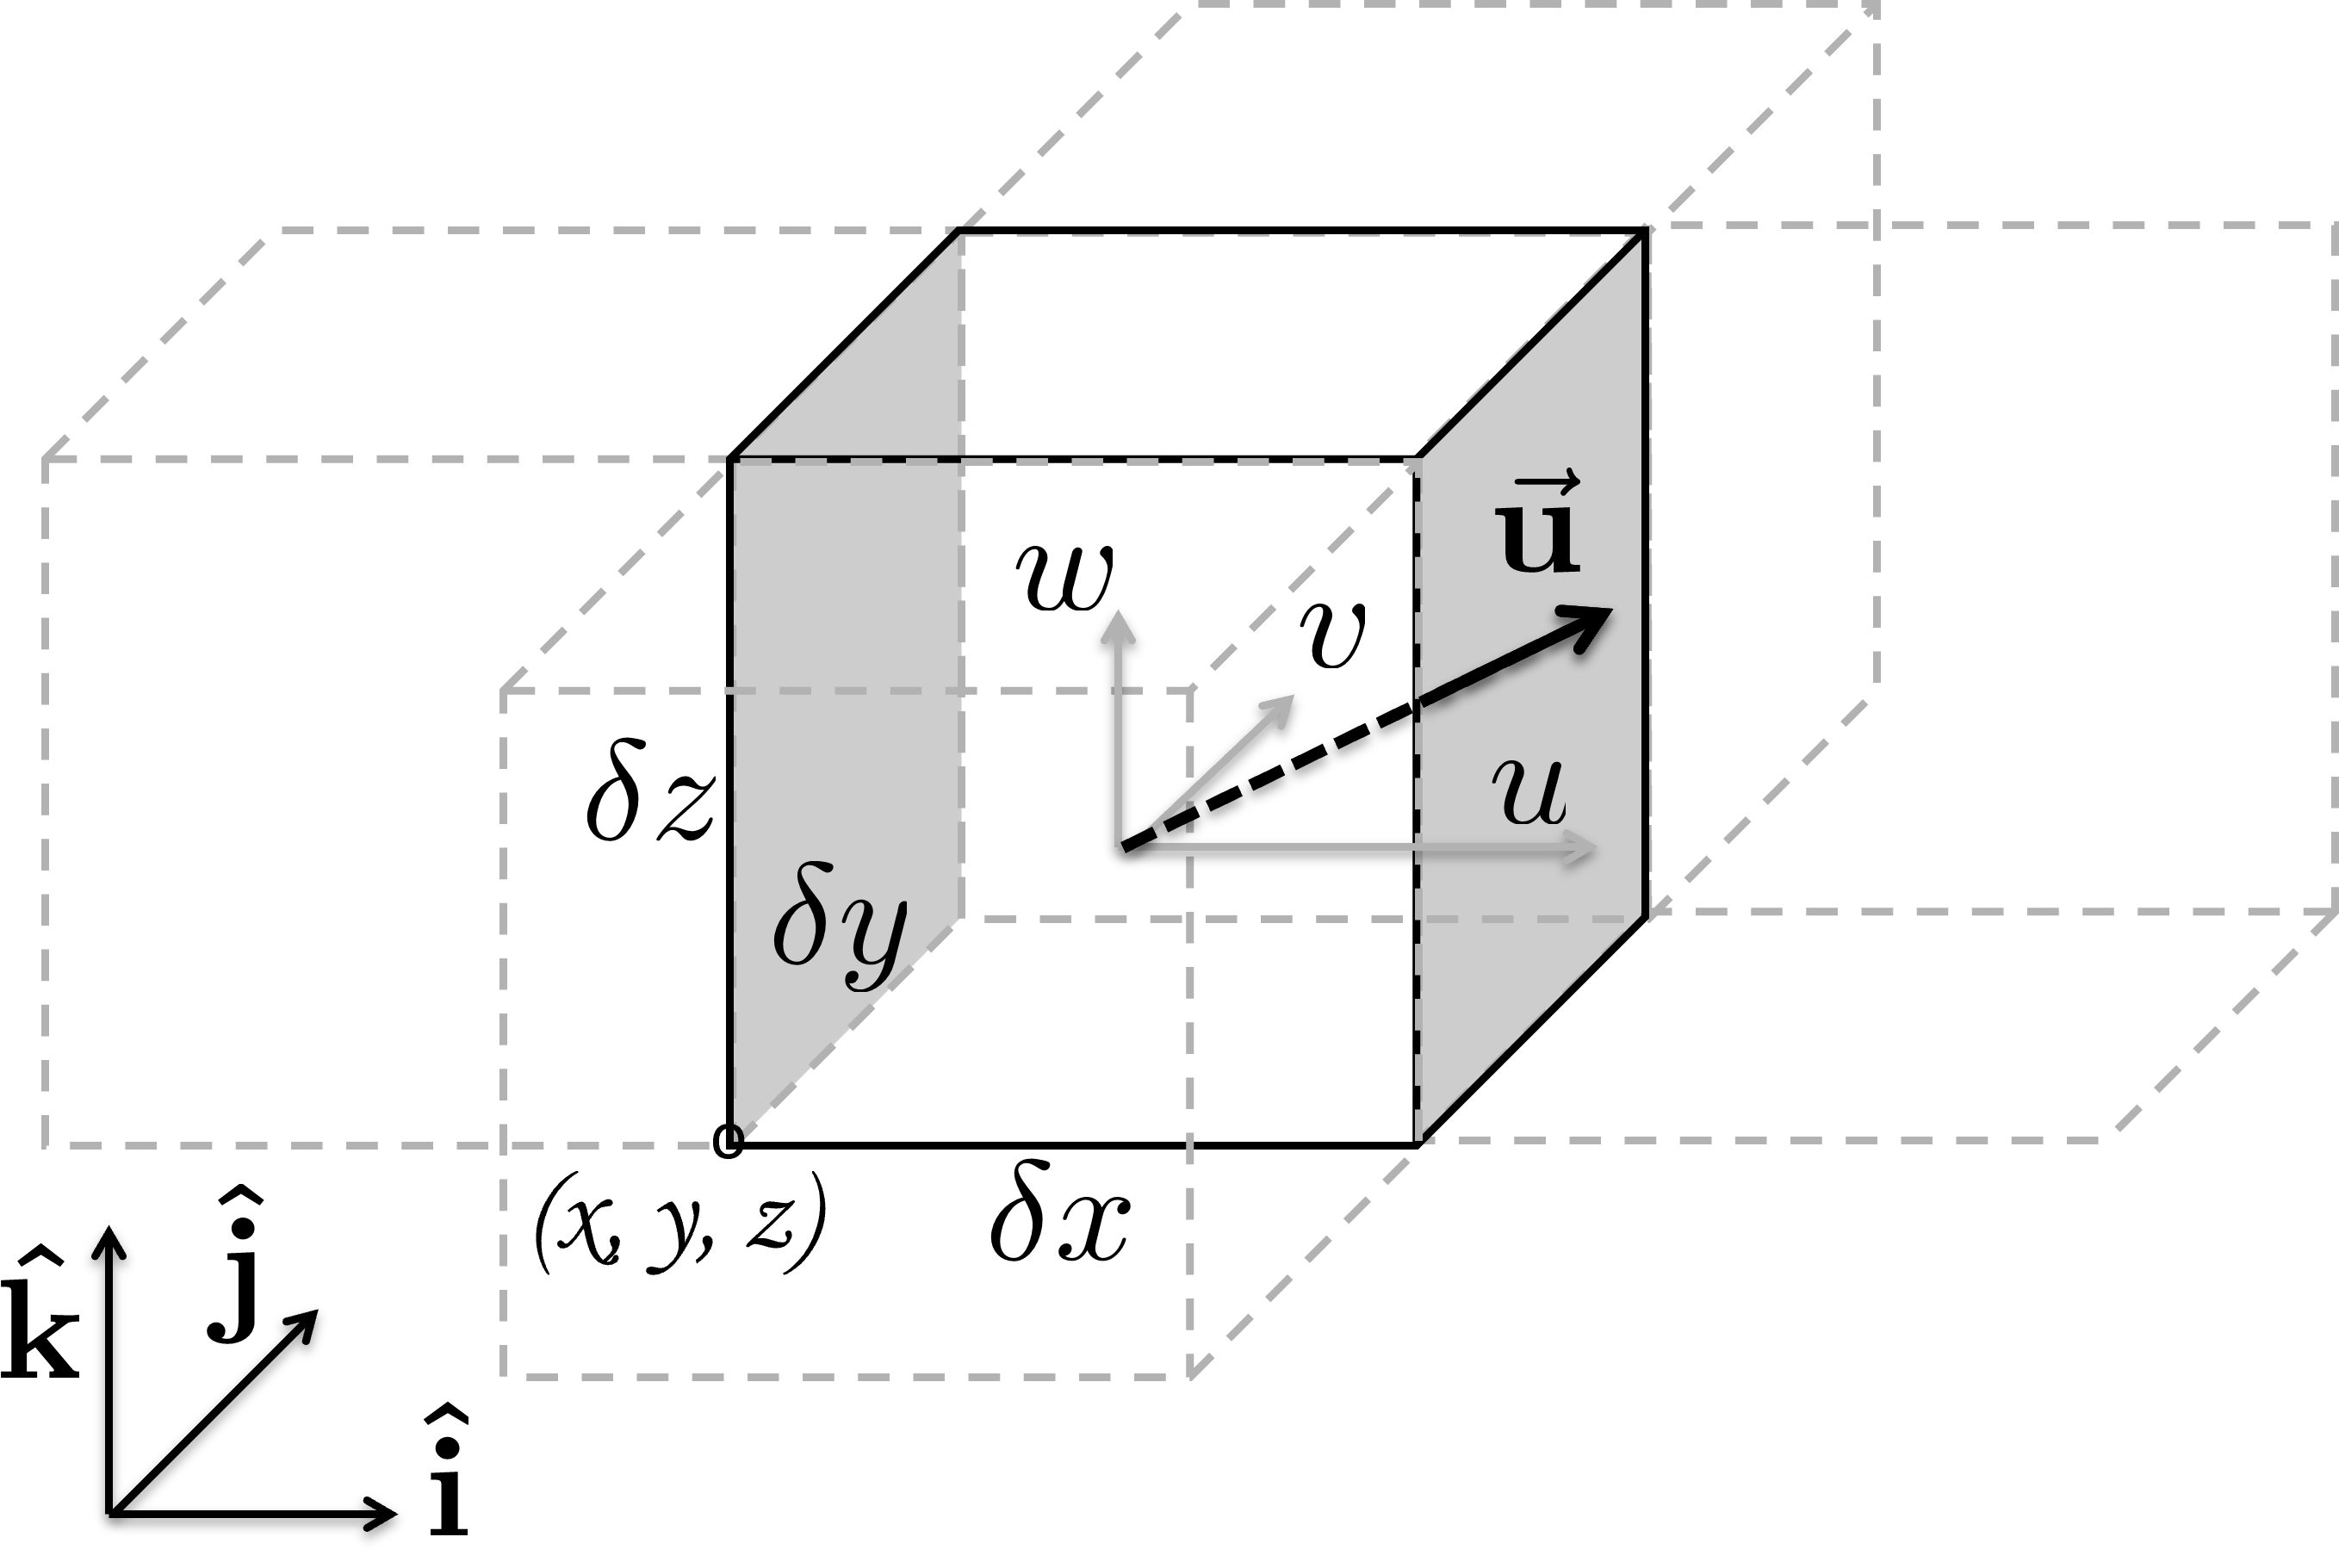
\includegraphics[width=6cm]{figures/M3/cube_control_volume}

{\small{}Our fluid parcel is a small cubic }\emph{\small{}control}{\small{}
}\emph{\small{}volume}{\small{} $\delta M=\rho\,\delta V$ with density
$\rho(x,y,z)$, volume $\delta V=\delta x\delta y\delta z$ and subjected
to the velocity field $\mathbf{u}=\left(u,v,w\right)$. By convention,
the origin is set in the lower left corner at point $\left(x,y,z\right)$,
but it can also be located in the centre of the box where we have
put the velocity vector }{\small\par}

\column{6cm}
\begin{itemize}
\item {\small{}The combination of forces acting on the volume follows Newton's
first and second laws
\begin{equation}
\sum\mathbf{F}=\delta M\,\mathbf{a}=\rho\delta V\,\frac{D\mathbf{u}}{Dt}\label{eq:newton-laws}
\end{equation}
where we use the total derivative because the parcel is part of a
moving fluid}{\small\par}
\item {\small{}The forces we consider are due to:}

\begin{itemize}
\item {\small{}gravity (internal to the parcel)}{\small\par}
\item {\small{}pressure (external)}{\small\par}
\item {\small{}friction (external)}{\small\par}
\end{itemize}
\end{itemize}
\end{columns}

\end{frame}


\section{Effects of gravity}
\begin{frame}{The gravity term}

\begin{columns}[t]


\column{7cm}
\begin{itemize}
\item The effect of gravity is independent of geometric considerations and
only based on the mass of the infinitesimal volume $\delta M=\rho\,\delta V$
\item It is directed downward (along the unit vector $\mathbf{\hat{k}}$)
using the gravitational constant
\begin{equation}
\mathbf{F}_{g}=-g\delta M\mathbf{\hat{k}}=-g\,\rho\,\delta V\,\mathbf{\hat{k}}
\end{equation}
\end{itemize}

\column{7cm}

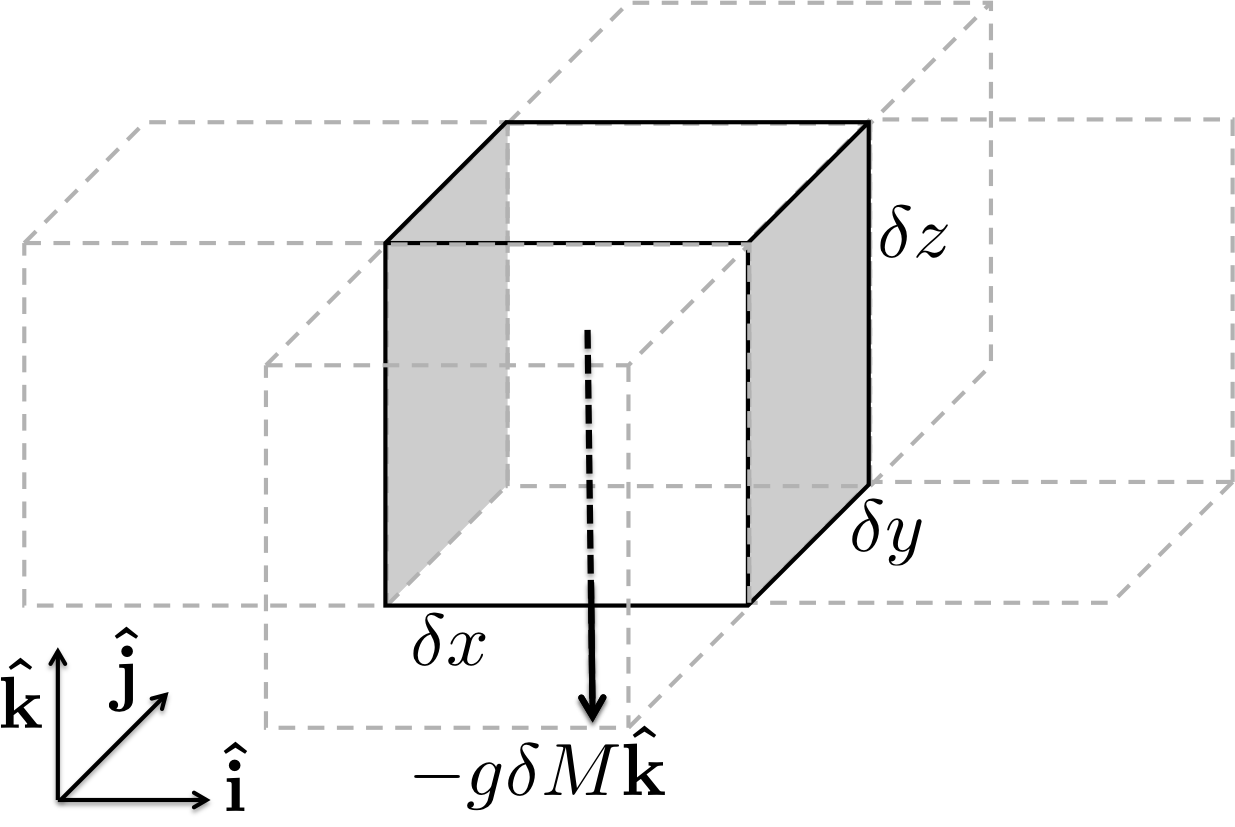
\includegraphics[width=7cm]{figures/M3/cube_gravity_term}
\end{columns}

\end{frame}


\section{Forces due to pressure}
\begin{frame}{The pressure gradient force}

\begin{columns}[t]


\column{7.5cm}
\begin{itemize}
\item {\small{}The geometry for computing the pressure force term is similar
to the derivation of the hydrostatic balance (see M2). }\textbf{\small{}Pressure
is isotropic}{\small{}: acts in all directions }{\small\par}
\item {\small{}We first compute the terms in the $x$ direction. The pressures
on the 2 faces are $p(x)$ and $p\left(x+\delta x\right)=p+\delta p$}{\small\par}
\item {\small{}The x-component along $\boldsymbol{\hat{i}}$ is written
considering the area of both sides 
\begin{align}
F_{p}^{x} & =p\left(x\right)\delta y\delta z-\left[p(x)+\frac{\partial p}{\partial x}\delta x\right]\delta y\delta z=\nonumber \\
 & =-\frac{\partial p}{\partial x}\delta x\,\delta y\,\delta z=-\frac{\partial p}{\partial x}\delta V\label{eq:pressure_gradient_x}
\end{align}
}{\small\par}
\end{itemize}

\column{6cm}

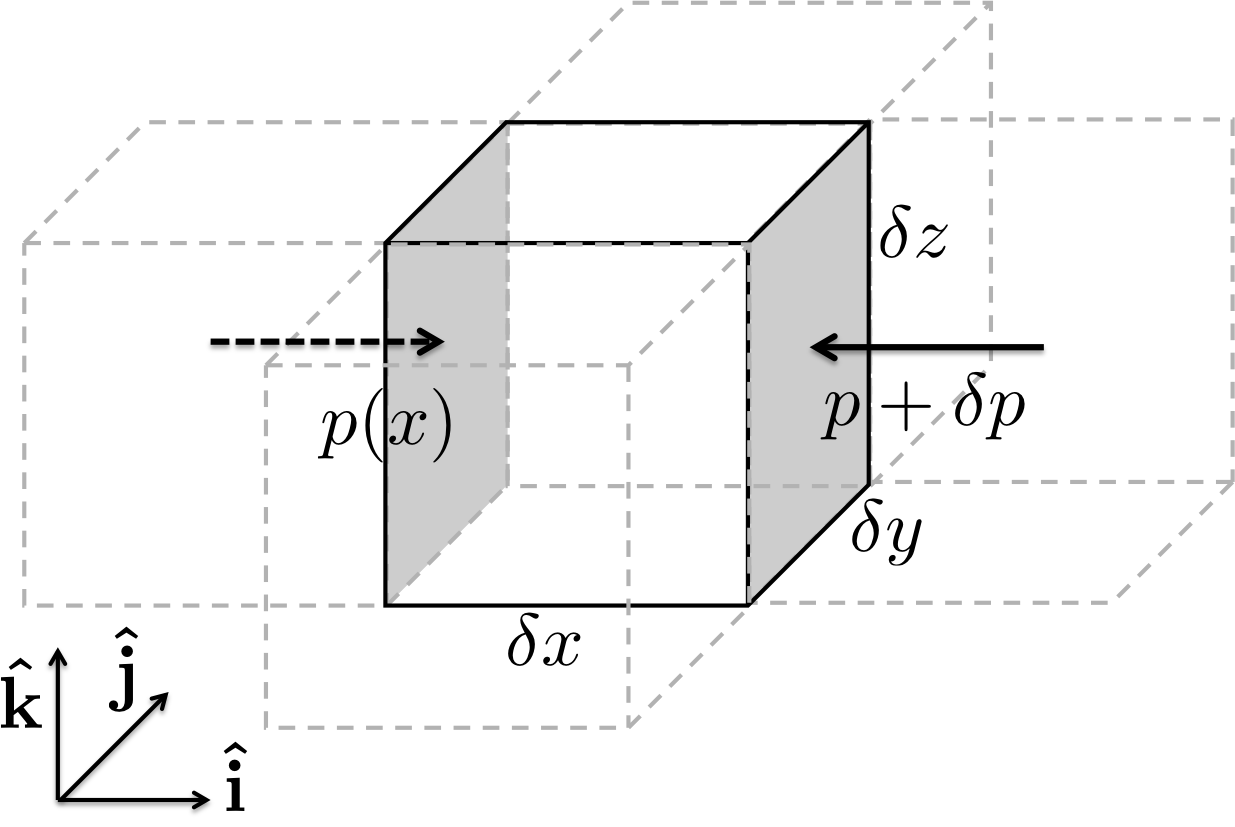
\includegraphics[width=6cm]{figures/M3/cube_pressure_term}

~{\footnotesize{}The change in pressure can be thought of in two
ways:}{\footnotesize\par}
\begin{enumerate}
\item {\footnotesize{}Using the differential along $x$: $\delta p=\partial p/\partial x\,\delta x$}{\footnotesize\par}
\item {\footnotesize{}With a Taylor series: $p\left(x+\delta x\right)=p(x)+\partial p/\partial x\,\delta x+\mathcal{O}\left(\delta x^{2}\right)$}{\footnotesize\par}
\end{enumerate}
\end{columns}

\end{frame}

\begin{frame}{The 3D pressure gradient term }

\begin{itemize}
\item We apply the same procedure shown in eq. (\ref{eq:pressure_gradient_x})
to all the sides of the parcel to get the components of the pressure
force
\begin{align*}
F_{p}^{x} & =-\frac{\partial p}{\partial x}\delta V\\
F_{p}^{y} & =-\frac{\partial p}{\partial y}\delta V\\
F_{p}^{z} & =-\frac{\partial p}{\partial z}\delta V
\end{align*}
\item We can write it in vector form by means of the nabla (\emph{del})
operator
\begin{equation}
\mathbf{F}_{p}=\left\langle F_{p}^{x},F_{p}^{y},F_{p}^{z}\right\rangle =-\left\langle \frac{\partial p}{\partial x},\frac{\partial p}{\partial y},\frac{\partial p}{\partial z}\right\rangle \delta V=-\boldsymbol{\nabla}p\,\delta V
\end{equation}
\item If the pressure is equal on all the opposing sides the gradient is
zero and there is no net force
\end{itemize}
\end{frame}


\section{Friction}
\begin{frame}{The concept of friction}

\begin{center}
\vspace{-0.5cm}
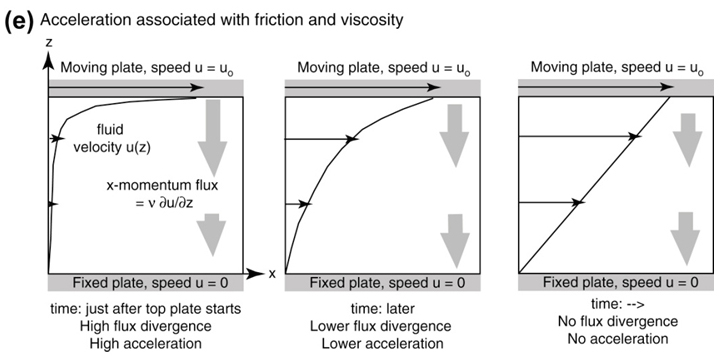
\includegraphics[scale=0.6]{figures/M3/viscous_forces_talley}
\par\end{center}
\begin{itemize}
\item \vspace{-0.5cm}
{\scriptsize{}We are somehow familiar with the concept of friction.
It is due to molecules rubbing against each other (}\textbf{\scriptsize{}molecular
viscosity}{\scriptsize{}) and to the transfer of motion through larger
parcels, which we call }\textbf{\scriptsize{}turbulence}{\scriptsize{}.
The acceleration of a parcel depends on the friction with the surrounding
parcels. Friction is due to the changes in the viscous }\textbf{\scriptsize{}stress}{\scriptsize{}
from one point to another, as we will see later in the course. }{\scriptsize\par}
\item {\scriptsize{}The figure above illustrates the momentum transfer from
a plate that is set into motion at the surface of a fluid until the
equilibrium flow is reached. At the beginning, the vertical gradient
of velocity is large, generating a large acceleration. After a while
the velocity propagates in the interior of the fluid and the acceleration
decreases due to the presence of the opposing frictional force. }{\scriptsize\par}
\end{itemize}
\end{frame}

\begin{frame}{Frictional forces}

\begin{columns}[t]


\column{6cm}
\begin{itemize}
\item At this stage we will not quantify the form of the frictional forces:
it's a term that includes viscous forces and turbulence dynamics
\item Friction has no preferential direction in space
\item Newton proposed that frictional forces are affected by the density
of the fluid
\begin{equation}
\mathbf{F}_{f}=\boldsymbol{\mathcal{F}}\delta M=\boldsymbol{\mathcal{F}}\rho\,\delta V
\end{equation}
\end{itemize}

\column{6cm}

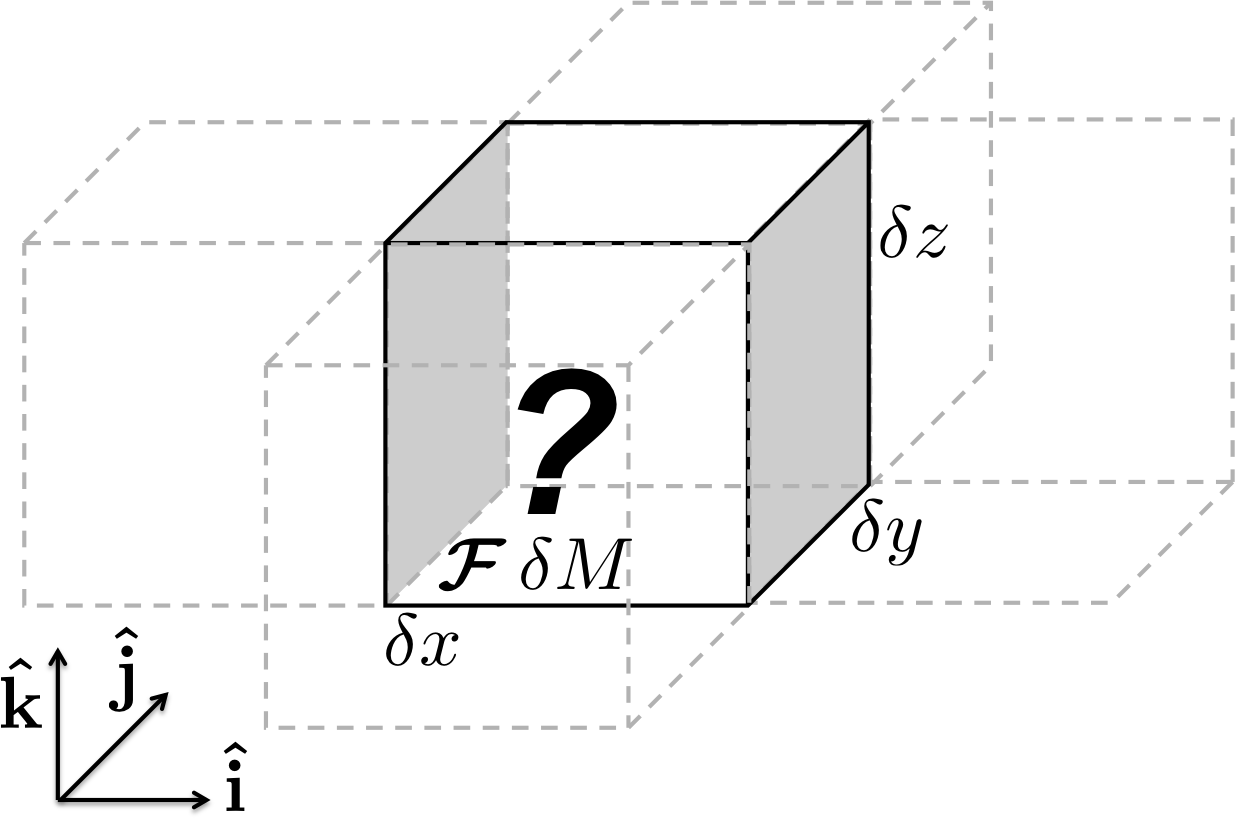
\includegraphics[width=6cm]{figures/M3/cube_friction_term}
\end{columns}

\end{frame}


\section{The Navier-Stokes equations}
\begin{frame}{The Navier-Stokes equations}

\begin{itemize}
\item Combining all the terms together using the formula shown in (\ref{eq:newton-laws})
we write 
\[
\rho\,\delta V\,\frac{D\mathbf{u}}{Dt}=\mathbf{F}_{pressure}+\mathbf{F}_{gravity}+\mathbf{F}_{friction}
\]
\item Substituting the expressions of each force with the proper signs yields
\[
\rho\,\delta V\,\frac{D\mathbf{u}}{Dt}=-\boldsymbol{\nabla}p\,\delta V-g\,\rho\,\delta V\,\mathbf{\hat{k}+\rho\boldsymbol{\mathcal{F}}}\delta V
\]
in which we notice that the volume (i.e. the shape of the parcel)
does not play any role. This is the general form of the equation of
motion for a fluid in a static system: \textbf{the Navier-Stokes equation}
(note that the bold nabla is dropped for ease of notation):
\begin{equation}
\boxed{\frac{D\mathbf{u}}{Dt}=-\frac{\nabla p}{\rho}-g\,\mathbf{\hat{k}}+\boldsymbol{\mathcal{F}}}
\end{equation}
\end{itemize}
\end{frame}

\begin{frame}{The components of the equation}

\begin{itemize}
\item Remembering the definition of the \textbf{total derivative} (M3.2),
the vector rules explained in the previous sections, and the vector
form of the equation you can always derive the components of the Navier-Stokes
in the 3 directions. The shape of the friction term will be made explicit
in a later section.
\begin{align*}
\frac{\partial u}{\partial t}+u\frac{\partial u}{\partial x}+v\frac{\partial u}{\partial y}+w\frac{\partial u}{\partial z} & =-\frac{1}{\rho}\frac{\partial p}{\partial x}+\mathcal{F}_{x}\\
\frac{\partial v}{\partial t}+u\frac{\partial v}{\partial x}+v\frac{\partial v}{\partial y}+w\frac{\partial v}{\partial z} & =-\frac{1}{\rho}\frac{\partial p}{\partial y}+\mathcal{F}_{y}\\
\frac{\partial w}{\partial t}+u\frac{\partial w}{\partial x}+v\frac{\partial w}{\partial y}+w\frac{\partial w}{\partial z} & =-\frac{1}{\rho}\frac{\partial p}{\partial z}-g+\mathcal{F}_{z}
\end{align*}
\end{itemize}
\end{frame}

\end{document}
